% ----------------------------------------------------------------------------
\chapter{Analysis and Comparision of Chat Systems}
%%    1. Detailed analysis and comparison of open and legacy chat systems
%%        to summarise current chat system features and their
%%        security characteristics.
% ----------------------------------------------------------------------------
\section{Internet Relay Chat (IRC)}
\subsection{History}
IRC has been developed since 1989, but was first formally documented in May 1993 in 
RFC 1459. It is still widely being used as of today.\cite{rfc1459,ircusage}
The current protocol is specified in the RFCs 2810-2813.\cite{rfc2810,rfc2811,rfc2812,rfc2813}
%%\begin{quote}
%%All client-to-server IRC protocols in use today are descended from the protocol implemented in the irc2.4.0 version of the IRC2 server, and documented in RFC 1459. Since RFC 1459 was published, the new features in the irc2.10 implementation led to the publication of several revised protocol documents (RFC 2810, RFC 2811, RFC 2812 and RFC 2813); however, these protocol changes have not been widely adopted among other implementations.\ref{irc-wp}
%%\end{quote}
% ----------------------------------------------------------------------------
\subsection{Architecture}
IRC is organised centrally, as stated in \cite{rfc2810}:
\begin{quote}
The IRC protocol provides no mean for two clients to directly
communicate.  All communication between clients is relayed by the
server(s).
\end{quote}
There is, however, an unofficial client extension named 
\textit{Direct Client-to-Client (DCC)} available in most IRC clients
that enables direct connections.\footnote{See \cite{dcc}, \cite{ctcp}.}
Figure \ref{ircoverview} shows the schematic overview of an IRC network.
\begin{figure}
    \caption{Schematic Overview of IRC}
    \label{ircoverview}
    \centering
    
    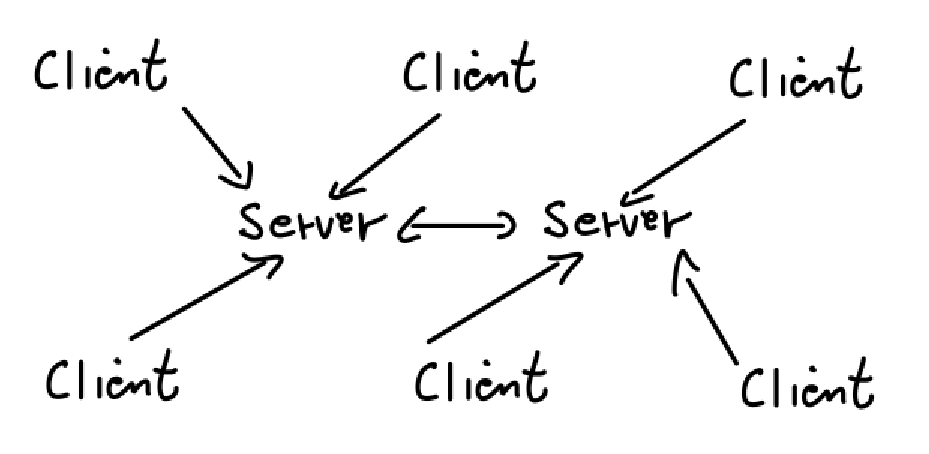
\includegraphics{irc.eps}
\end{figure}
IRC supports 
\textit{direct chat} (one peer to another peer) as well 
as \textit{group chat} (many peers to many peers). The group chat is
realised by creating \textit{IRC channels}, sometimes also called 
\textit{chat rooms}.
% ----------------------------------------------------------------------------
\subsection{Security}
The TLS protocol \cite{rfc2246} is being used in some networks,
but its use is not standardised. Connections from clients to servers
as well as servers to servers may be encrypted.
Some networks support special channel modes to ensure all connected peers
are connected using an encrypted connection. There is no such mode for
direct chat. For normal IRC channels, there is no guarantee that all
peers are connected using an encrypted connection.

Due to its architecture, every operator of a server can listen to all
messages, even if encryption is being used. As the network usually consists
of many clients, but only a small number of servers, an attacker needs
to concentrate on a small number of victim hosts only.

Usually IRC networks do not provide any kind of anonymisation features:
every user can request detailled information about other users, including
their IP address.  The freenode network\cite{freenode} however,
supports so called \textit{cloaks}, which transfer the IP address information
into a generic string like \textit{gpm/telmich}, in which gpm describe the
project and telmich the name. There are various other cloacking expressions
available
% ----------------------------------------------------------------------------
\section{Secure Internet Live Conferencing (SILC)}
% ----------------------------------------------------------------------------
\subsection{History}
The \textit{ecure Internet Live Conferencing (SILC)} protocol
has been developed by Pekka Riikonen since 1996. The first public release
has been made in 2000. The last releases of SILC software (server and client)
are dated at 2009. Silc can be considered a more secure successor of IRC,
as can be seen in the following quote:
\begin{quote}
\ldots{}
Many of the SILC features are found in traditional chat protocols such 
as IRC but many of the SILC features can also be found in 
Instant Message (IM) style protocols.

SILC combines features from both of these chat protocol styles, 
and can be implemented as either IRC-like system 
or IM-like system. \ldots{}\cite{silcwp}
\end{quote}
As far as the official website reports,
there is no version controlled source code repository available,
only tarballs from 2009 are downloadable. This may indicate that the
development of the SILC software has stagnated.
% The SILC Project's goal is to fully standardize the SILC protocol in the IETF. 
%Bug form does not return any bugs.
Besides the official SILC Network, which is run by 7 SILC servers,
there are about 12 other SILC networks being run.\cite{wiki:silc}
% ----------------------------------------------------------------------------
\subsection{Architecture}
Figure \ref{silcoverview} shows 
that SILC Network architecture looks similar to IRC network architecture: 
\begin{figure}
    \centering
    \caption[Schematic Overview of SILC]{Schematic Overview of SILC\\Image source: \protect\url{http://www.silcnet.org/img/silc_network.png}}
    \label{silcoverview}
    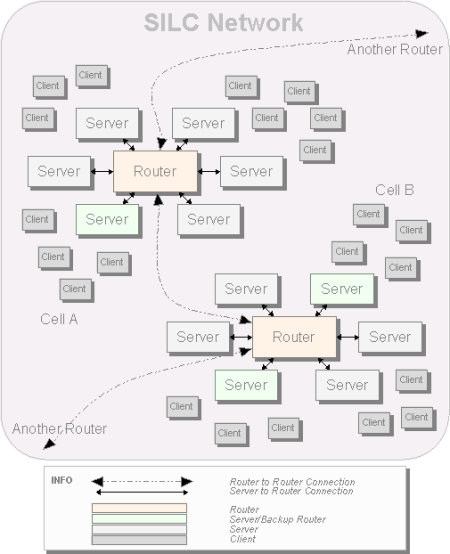
\includegraphics[scale=0.8]{silc_network.png}
\end{figure}
Both rely on a central design orientated on a network of servers.
In case of SILC, there are two different variants of message passing:
\begin{itemize}
\item Private Message Delivery With Session Keys
\item Private Message Delivery With Private Message Key
\end{itemize}
In any case, all messages are travelling through supporting servers and are never
transmitted directly from one to another client.
% ----------------------------------------------------------------------------
\subsubsection{Private Message Delivery With Session Keys}
When the silc client uses session keys, every message is send encrypted
with the session key of the next peer, decrypted at the peer and re-encrypted
for the next peer in the chain, as can be seen in figure \ref{silcsessionkey}.
\begin{figure}
    \centering
    \caption[Silc: Private Message Delivery With Session Keys]{Private Message Delivery With Session Keys\\Image source: \protect\url{http://www.silcnet.org/img/silc_priv1.png}}
    \label{silcsessionkey}
    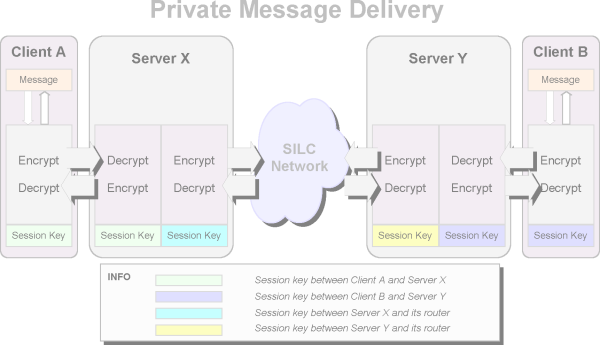
\includegraphics[scale=0.8]{silc_priv1.png}
\end{figure}
In this scenario, every peer in the communication chain
can read the content of the message.
% ----------------------------------------------------------------------------
\subsubsection{Private Message Delivery With Private Message Key}
When using a a private message key, the servers in the communication chain
only forward the message and the receiving peer is the only one who can
decrypt the message. Figure \ref{silcprivkey} illustrates this behaviour.
\begin{figure}
    \centering
    \caption[Silc: Private Message Delivery With Private Message Key]{Private Message Delivery With Private Message Key\\Image source: \protect\url{http://www.silcnet.org/img/silc_priv2.png}}
    \label{silcprivkey}
    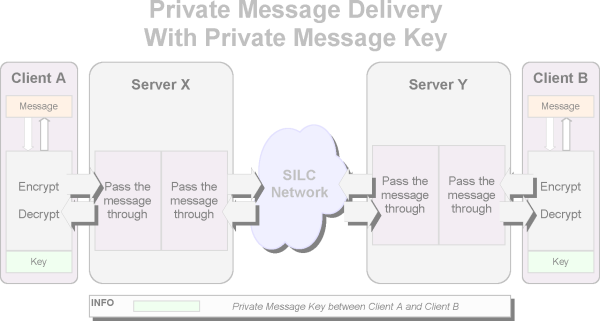
\includegraphics[scale=0.8]{silc_priv2.png}
\end{figure}
% ----------------------------------------------------------------------------
\subsection{Security}
As all messages in the SILC network are encrypted, an external attacker
cannot read the message content. In case Private message delivery with session keys
is utilised, a comproised SILC server may be used to intercept and read all
messages. This is not possible, if messages are sent using
private message delivery with private message key.
Due to the small number of servers (7 in the official network),
an attacker could run a \textit{Denial-of-Service (DoS)} attack to prevent
users from chatting.

The SILC network does not provide any kind of anonymity services and allows
to query detailled information about a peer including the IP address.
% ----------------------------------------------------------------------------
\section{Extensible Messaging and Presence Protocol (XMPP)}
% ----------------------------------------------------------------------------
\subsection{History}
The \textit{Extensible Messaging and Presence Protocol (XMPP}
was originally developed by Jeremie Miller in 1998 and released
to the public as \textit{Jabber} in 1999. In 2004 Jabber
was transfered to the IETF, renamed to XMPP
and is now defined in several
RFCs.\cite{rfc3920,rfc3921,rfc3922,rfc3923,rfc4622,rfc4854,rfc4979,rfc6120,rfc6121}
Since then, the \textit{XMPP Standards Foundation (XSF)} is responsible
for standardising XMPP related protocols, the so called 
\textit{XMPP Extension Protocols (XEP)}.
It is estimated that by 2003 XMPP has been used by 10 million people.\cite{xmppuser}
AOL added experimental support for XMPP in the 
\textit{AOL instant Messenger (AIM)} in 2008.
In 2010 the social-networking site Facebook added support for
third-party applications via XMPP.
As of 2012, there are over 30 different client and about 20
server implementations available.
% ----------------------------------------------------------------------------
\subsection{Architecture}
The XMPP network is built upon the ideas of e-mail: Users are identified
by e-mail alike usernames like \textit{nico@example.org}. The clients and
servers of the network find the correct server to talk to by making an
DNS SRV\cite{rfc2782} lookup. 
Clients are asking for the \textit{xmpp-client} service
servers are asking for the \textit{xmpp-server} service.
Thus a client thus may ask for a SRV record
\url{_xmpp-client._tcp.example.net.} or a server for
\url{_xmpp-server._tcp.im.example.com.}
If there is no SRV record, the client or server can fall back
to request for the A or AAAA record, similar to how 
SMTP\cite{rfc2821} behaves. Figure \ref{jabberarch} shows
how the client \textit{nico@example.org} sends a message
to \textit{nico@example.net}.
\begin{figure}
    \centering
    \caption{XMPP Network Architecture}
    \label{jabberarch}
    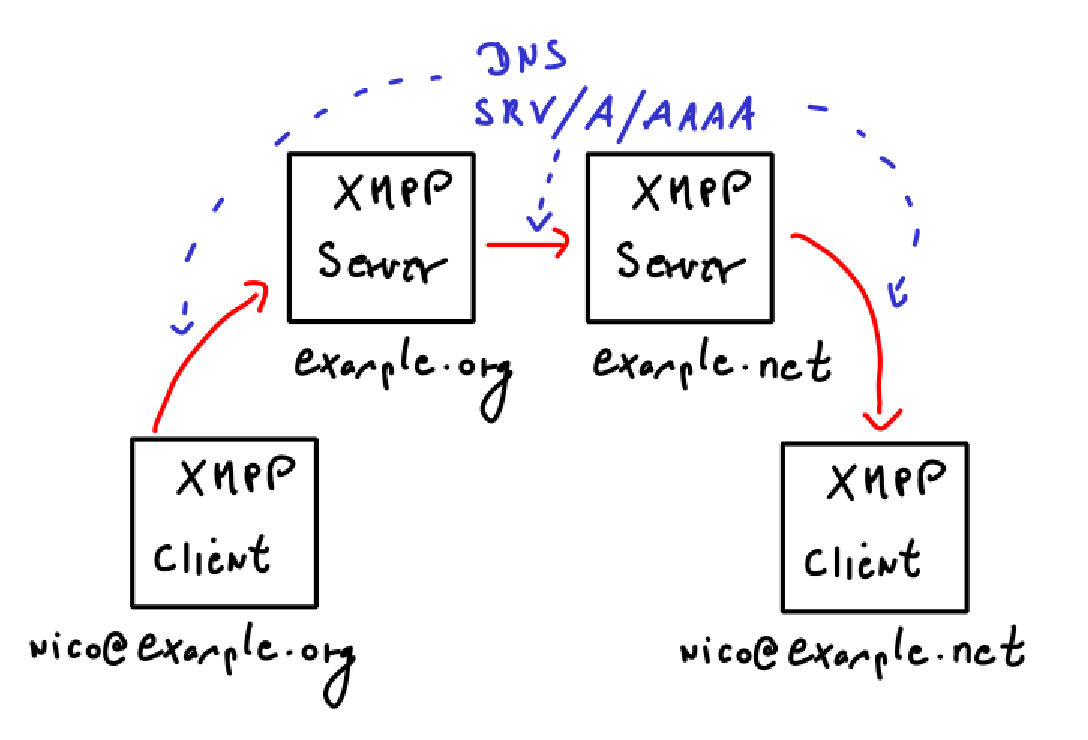
\includegraphics[scale=0.8]{jabberarch.eps}
\end{figure}
XMPP formats messages based on the 
\textit{Extensible Markup Language (XML)} and
supports authentication using a 
Simple Authentication and Security Layer (SASL)\cite{rfc4422}.
Clients never talk directly to each other in a XMPP network, but
always use one or more servers in between. Compared to IRC and SILC,
XMPP is the only protocol that supports connecting other protocols
like AIM or IRC.
% ----------------------------------------------------------------------------
\subsection{Security}
Within XMPP TLS is being used for encryption 
and SASL for authentication.
XMPP does not have mechanism to support anonymity.
To create a DoS attack, an attacker can choose to take either the sending
or the receiving server down. Due to its openess, an attacker can find out
which server she needs to attack by doing DNS queries. Though when attacking
the sending server, the sending client can just switch to another server,
as figure \ref{jabbersendingserverattack} shows.
\begin{figure}
    \centering
    \caption{XMPP Sending Server Attack}
    \label{jabbersendingserverattack}
    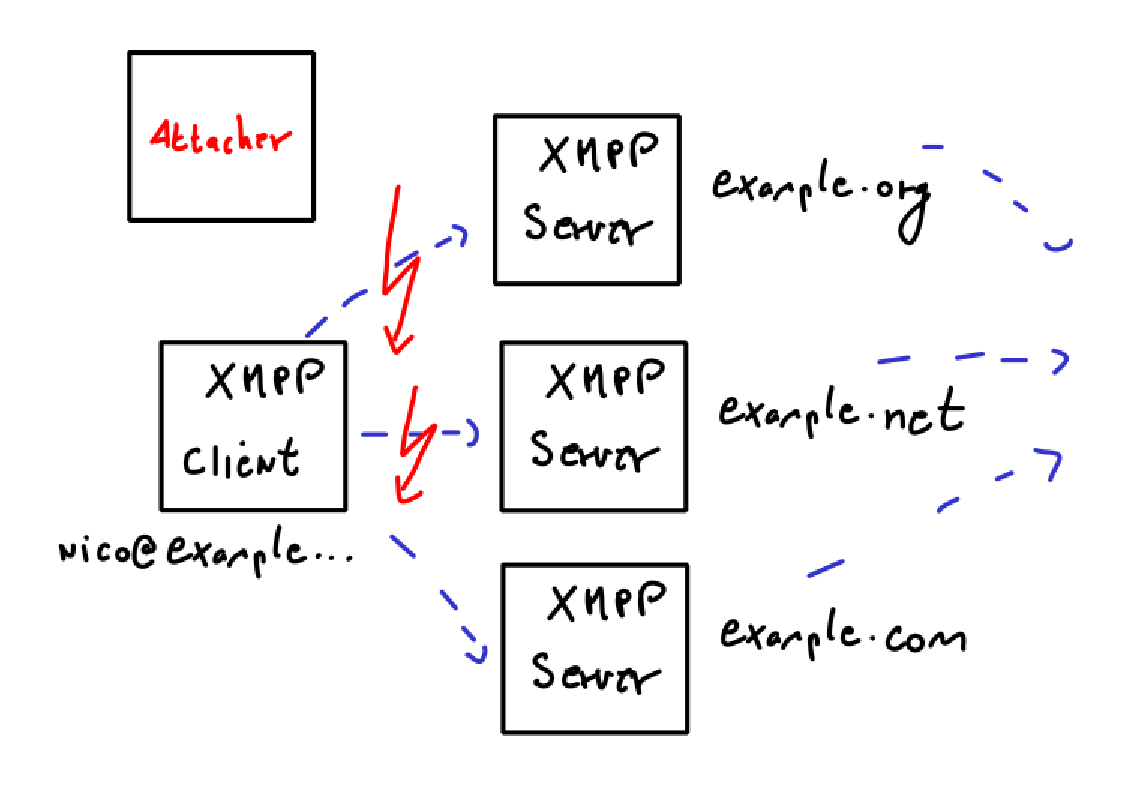
\includegraphics[scale=0.7]{jabbersendingserverattack.eps}
\end{figure}
If the attacker aims to bring down the receiving server, the message
will not arrive while the server is down, as shown in figure 
\ref{jabberreceivingserverattack}.
\begin{figure}
    \centering
    \caption{XMPP Receiving Server Attack}
    \label{jabberreceivingserverattack}
    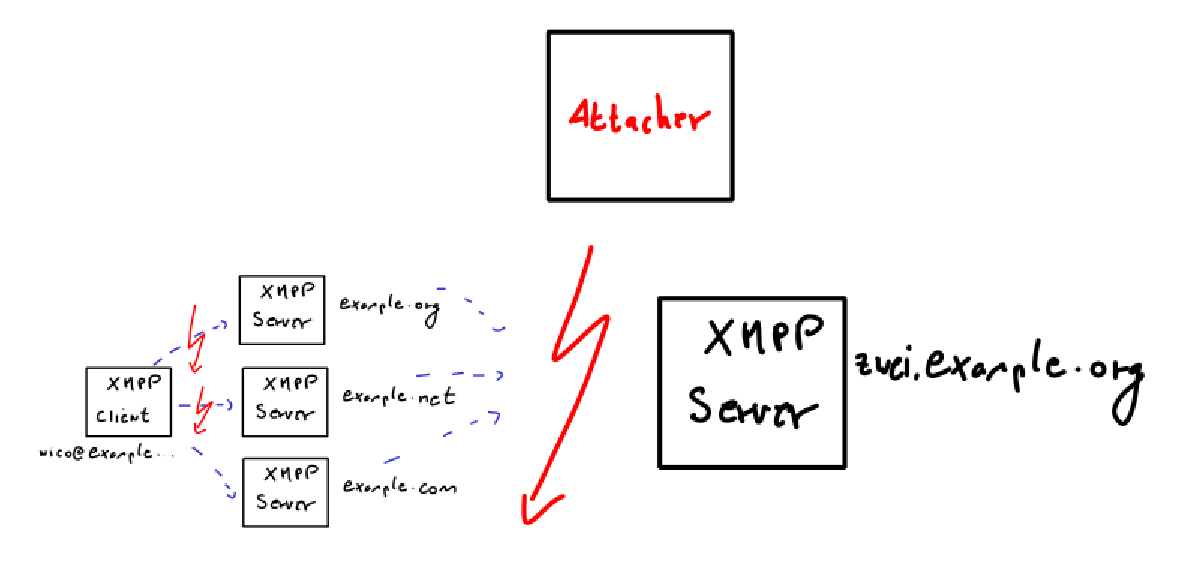
\includegraphics[scale=0.7]{jabberreceivingserverattack.eps}
\end{figure}
% ----------------------------------------------------------------------------
\section{Skype}
% ----------------------------------------------------------------------------
\subsection{History}
% ----------------------------------------------------------------------------
\subsection{Architecture}
% ----------------------------------------------------------------------------
\subsection{Security}

% ----------------------------------------------------------------------------
\section{Other}
There are further chat protocols, which have not been included into this
analysis, either because of known weaknesses, irrelevance or small user base.
ICQ, which has been published in 1996, is not being widely used anymore
and its protocol, OSCAR\cite{oscar}, is based on plain text messages.
ICQ used to be popular, but has been sold to the russian Mail.ru group.

MSN

% ----------------------------------------------------------------------------
\section{Security features and Comparision}

\begin{longtable}{|c|c|c|}
\caption{Chat system comparision with security features}\\
\hline
\textbf{Name} & \textbf{IRC} & \textbf{SILC}\\
\hline
\textbf{Single point of attack} & yes & yes\\
\hline
\textbf{Encrypted traffic} & optional & yes\\
\hline
\end{longtable}

All the solutions with objectives.
